\documentclass[aps]{revtex4}
\usepackage{graphicx}
\usepackage{amssymb,amsfonts,amsmath,amsthm}
\usepackage{chemarr}
\usepackage{bm}
\usepackage{pslatex}
\usepackage{mathptmx}
\usepackage{xfrac}

%% concentration notations
\newcommand{\mymat}[1]{\boldsymbol{#1}}
\newcommand{\mytrn}[1]{{#1}^{\mathsf{T}}}
\newcommand{\myvec}[1]{\overrightarrow{#1}}
\newcommand{\mygrad}{\vec{\nabla}}
\newcommand{\myhess}{\mathcal{H}}



\begin{document}
\title{Differential Bubbles}
\maketitle

\section{Differential Properties}

\subsection{Tangent Field}
Let us assume that we have three vectors $\vec{M}_-$, $\vec{M}_0$ and $\vec{M}_+$, with
$t_-=\left\vert \myvec{M_0M_-}\right\vert$ and $t_+=\left\vert \myvec{M_0M_+}\right\vert$.
The regular curve approximation is
\begin{equation}
	\vec{M}(t) = \vec{M}_0 + t \partial_t \vec{M} + \frac{1}{2} t^2 \partial_{t}^2 \vec{M}
\end{equation}
so that
\begin{equation}
\left\lbrace
\begin{array}{rcl}
	\myvec{M_0M_-} & = & -t_- \partial_t \vec{M} + \frac{1}{2} t_-^2 \partial_{t}^2 \vec{M}\\
	\myvec{M_0M_+} & = &  t_+ \partial_t \vec{M} + \frac{1}{2} t_+^2 \partial_{t}^2 \vec{M}.\\
\end{array}
\right.
\end{equation}
Setting

\begin{equation}
\left\lbrace
\begin{array}{rcl}
	\vec{V}_- & = & \frac{1}{t_-} \myvec{M_0M_-}\\
	\vec{V}_+ & = & \frac{1}{t_+} \myvec{M_0M_+}\\
\end{array}
\right.
\end{equation}
we shall solve
\begin{equation}
	\left\lbrace
	\begin{array}{rcl}
	\vec{V}_- & = & -\partial_t \vec{M} + \frac{1}{2} t_- \partial_{t}^2 \vec{M}\\
	\vec{V}_+ & = & \partial_t \vec{M} + \frac{1}{2} t_+ \partial_{t}^2 \vec{M}.\\
	\end{array}
\right.
\end{equation}

The first order approximation of the tangent field is
\begin{equation}
	\partial_t \vec{M} =  \frac{1}{t_-+t_+} \left(t_-\vec{V}_+ - t_+ \vec{V}_-\right)
\end{equation}

\subsection{Differential properties}
Let us assume that $\vec{M}(t)$ is a local parametric estimation of a contour.
Then the tangent vector around $\vec{M}_0$ is
\begin{equation}
	\partial_t \vec{M} = 
	 \frac{1}{t_-+t_+} \left\lbrack t_-\left(\frac{1}{t_+}\myvec{M_0M_+}\right) - t_+ \left(\frac{1}{t_-}\myvec{M_0M_-}\right)\right\rbrack
\end{equation}
and the tangent vector is
\begin{equation}
	\vec{\tau} = \frac{1}{\vert \partial_t \vec{M} \vert} \partial_t \vec{M}
\end{equation}
and the normal vector is
\begin{equation}
	\vec{n} = \begin{bmatrix}
		-\tau_y\\
		\tau_x\\
	\end{bmatrix}.
\end{equation}
If $s$ were a curvilinear abscissa then we would have
\begin{equation}
	\partial_s \vec{\tau} = \kappa \vec{n}
\end{equation}
so that
\begin{equation}
	\kappa = \frac{1}{\vert\partial_t \vec{M}\vert} \vec{n}.\partial_t \vec{\tau}
\end{equation}
with
\begin{equation}
	\partial_t \vec{\tau} = \frac{1}{t_-+t_+}
	 \left\lbrack 
	 t_-\left(\frac{1}{t_+}\left(\vec{\tau}_+ - \vec{\tau}_0\right)\right) 
	- 
	t_+ \left(\frac{1}{t_-}\left(\vec{\tau}_- - \vec{\tau}_0\right)\right)
	\right\rbrack.
\end{equation}

So that the differential properties can be determined in two passes:
\begin{enumerate}
	\item Estimate $\partial_t \vec{M}$, deduce $\vec{\tau}$ and $\vec{n}$, and store $\vert\partial_t \vec{M}\vert$,
	\item then estimate $\partial_t \vec{\tau}$ and deduce $\kappa = \frac{1}{\vert\partial_t \vec{M}\vert} \vec{n}.\partial_t \vec{\tau}$.
\end{enumerate}

\section{Segmentation}
\subsection{Computing Junctions with a Grid}

To be sure that a vector between to consecutive tracers has only ONE intersection with an horizontal or a vertical
grid, we must ensure that this distance is less than $\lambda=\min(\delta x_i,\delta y_j)/2$.

\begin{center}
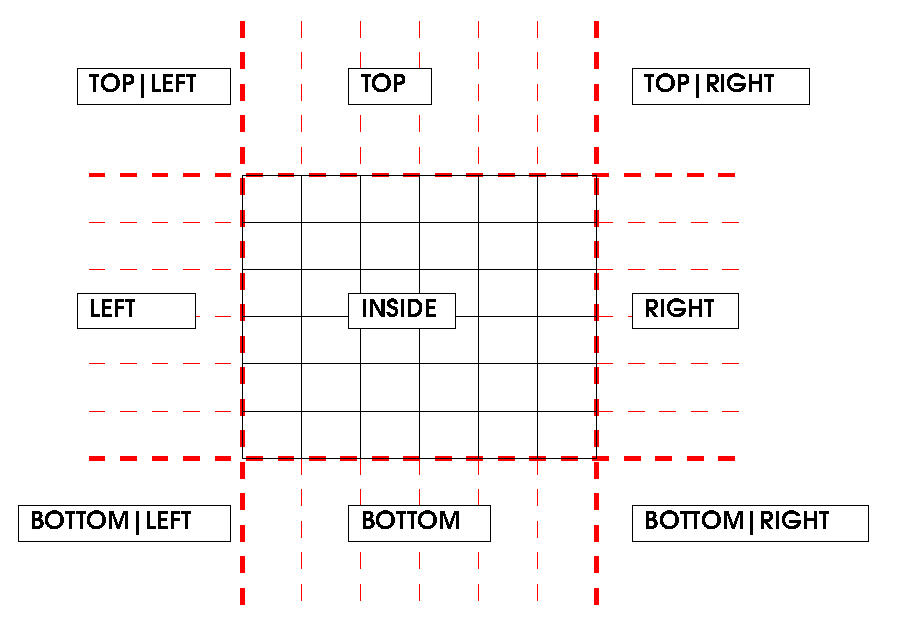
\includegraphics[scale=1]{grid.eps}
\end{center}

There is an intersection with an Horizontal axis if one of the point is Not in TOP and Not in BOTTOM and
\begin{itemize}
	\item the other point is in TOP or in BOTTOM
	\item or the other point is between two different horizontal axis (i.e. directly above or below).
\end{itemize}

There is an intersection with a Vertical axis if one of the point is Not in LEFT and Not in RIGHT and
\begin{itemize}
	\item the other point is in LEFT or in RIGHT
	\item or the other point is between to different vertical axis (i.e. directly at left or at right). 
\end{itemize}

\subsection{Segmentation by Ray Casting}
For non penetrating bubbles, the successive junctions pairs on any axis is the sequence of inside/outside positions.
When those junctions are within the grid (taking special care of sides), we mark the inner position with the owning bubble ID.

\section{Effective Pressure Field}
We need to estimate the pressure gradient and Laplacian around any bulk position,
using the \textbf{standard} discretizations.

\subsection{Entering Pressure Fields}
Let us assume that the points $x_{i-1}$ and $x_i$ are in the bulk, and that there is
an intersection with a bubble at $x_i+\phi$.
The length of the segment
is
$$
	L = \delta_x + \phi.
$$ 
At this intersection, there is a pressure $P_\phi = P_{bubble} - \gamma \kappa_\phi$.
The pressure gradient while \textbf{entering} the bubble can be estimated by
$$
	\sigma = \dfrac{P_\phi - P_{i-1}}{L}.
$$
We can define an \textbf{Order 1 Entering Pressure} $P^{E_1}$ by
$$
	\sigma = \dfrac{P^{E_1}_{i+1}-P_{i-1}}{2\delta_x} 
$$
so that
$$
	P^{E_1}_{i+1} = P_{i-1} + 2\delta_x\sigma.
$$
Using $h= \dfrac{L}{2}$, the pressure at the middle of the segment can be expressed as
$$
	P_{i,m}^E = \dfrac{1}{\delta_x} \left\lbrack
	h P_i + \left(\delta_x - h\right) P_{i-1}
	\right\rbrack
$$
We can define an \textbf{Order 2 Entering Pressure} $P^{E_2}$ by
$$
	\partial_x^2 P_i = \dfrac{P_{i-1} - 2P_{i,m}^E + P_\phi}{{h}^2} = \dfrac{P_{i-1}- 2P_i + P_{i+1}^{{E_2}}}{\delta_x^2}
$$
so that
$$
	P_{i+1}^{{E_2}} = 2P_i - P_{i-1} + \left(\dfrac{\delta_x}{h}\right)^2
	\left(
		P_{i-1} - 2P_{i,m}^E + P_\phi
	\right)
$$
The contribution to the Gauss-Seidel Method is
$$
	-\dfrac{2}{h\delta_x}
$$

\subsection{Leaving Pressure Fields}
Let us assume that  the points $x_{i}$ and $x_{i+1}$ are in the bulk, and that
theres is an intersection with a bubble at $x_i-\psi$.
At this intersection, there is a pressure $P_\psi=P_{bubble} - \gamma \kappa_\psi$.
The length of the segment is
$$
	L = \psi+\delta_x
$$
The pressure gradient while \textbf{leaving} the bubble can be estimated by
$$
	\sigma = \dfrac{P_{i+1}-P_\psi}{L}.
$$
We can define an \textbf{Order 1 Leaving Pressure} $P^{L_1}$ by
$$
	\sigma = \dfrac{P_{i+1}-P^{L_1}_{i-1}}{2\delta_x}
$$
so that 
$$
	P^{L_1}_{i-1} = P_{i+1} - 2\delta_x \sigma.
$$
Using $h = \dfrac{L}{2}$, the pressure at the middle of the segment can be estimated
by
$$
	P_{i,m}^L = \dfrac{1}{\delta_x} \left\lbrack
	h P_i + \left(\delta_x - h\right) P_{i+1}
	\right\rbrack.
$$
As previously, the \textbf{Order 2 Leaving Pressure} $P^{L_2}$ is
defined by
$$
	P_{i-1}^{L_2} = 2P_i - P_{i+1} + \left(\dfrac{\delta_x}{h}\right)^2
	\left(
		P_\psi - 2P_{i,m}^L + P_{i+1}
	\right)
$$
The contribution to the Gauss-Seidel weight is
$$
	-\dfrac{2}{\delta_x h}
$$

\subsection{Pinched Pressure Fields}
Let us assume that the point $x_i$ is between two bubbles at $x_i+\phi$ and $x_i-\psi$.
We have a segment length 
$$
	L = \phi + \psi 
$$
and a gradient
$$
	\sigma_i = \dfrac{P_\phi - P_\psi}{L}
$$
so that setting
$$
	P^{L_1}_{i-1} = \dfrac{2\delta_x}{L} P_\psi
$$
and
$$
	P^{E_1}_{i+1} = \dfrac{2\delta_x}{L} P_\phi
$$
solves the order 1 estimation.

We use $h=\frac{L}{2}$.
The pressure at the center of the pinch can be expressed like this.
\begin{itemize}
\item If $\phi>\psi$, 
$$
	P_{i,m} = \dfrac{1}{\phi}
	\left\lbrack
		h P_i + \left(\phi-h\right) P_\phi
	\right\rbrack
$$
\item If $\psi>\phi$,  
	$$
		P_{i,m} = \dfrac{1}{\psi}
	\left\lbrack
		h P_i + \left(\psi-h\right) P_\psi
	\right\rbrack
$$
\item Otherwise (numerically), $P_{i,m}=P_i$.
\end{itemize}

The the second derivative of the pressure is estimated by
$$
	\partial_x^2 P_i = \dfrac{P_\psi - 2P_{i,m} + P_\phi}{h^2} =
	\dfrac{P^{L_2}_{i-1} - 2P_i + P^{E_2}_{i+1}}{\delta_x^2}.
$$
We solve the order 2 problem by setting
$$
	P^{L_2}_{i-1} = P^{E_2}_{i+1} = P_i + \dfrac{1}{2}\left(\dfrac{\delta_x}{h}\right)^2 \left( P_\psi - 2P_{i,m} + P_\phi \right)
$$
The contribution to the Gauss-Seidel algorithm are the following
\begin{itemize}
	\item If $\phi>\psi$, it is
	$$
		-\dfrac{2}{h\phi}
	$$
	\item If $\psi>\phi$, it is
	$$
		-\dfrac{2}{h\psi}
	$$
	\item Otherwise, it is 
	$$
		-\dfrac{2}{h^2}
	$$
\end{itemize}
\subsection{Conclusion}

\section{Adaptive Polygon}

\subsection{Problem}
On a grid, we want to remap a polygonized contour with a distance of about $\lambda$ between consecutive vertices.

\subsection{Reduction with Area Conservation}


\section{Local Gradient Estimation}

\subsection{Tangential Gradient}
If we have the contour $\vec{M}(t)$ and the corresponding $P(t)$, then
$$
	\partial_t P = \mygrad P , \partial_t M = \left(\mygrad P . \vec{\tau}\right) \left|\partial_t \vec{M}\right|.
$$

Accordingly, we compute $\partial_t P$ and we use the stored $\left|\partial_t \vec{M}\right|$.

\subsection{Normal Gradient}
\subsubsection{Constructing the Normal Pressure Field}

Let us assume that we have $q$ points $\vec{Q}_1,\ldots,\vec{Q}_{q}$ around a point $\vec{A}$, and that we want to
estimate the pressure gradient along the direction $\vec{u}$, $\vert\vec{u}\vert=1$. 
We also assume that we know the pressure gradients at each $\vec{Q}_i$.
Therefore, we need to compute the variation of pressure on the $(\vec{A},\vec{u})$ axis.
We estimate the pressure from a $\vec{Q}_i$ point by
$$
	\tilde{P}_i(\vec{M}) = P_i + \vec{G}_i.\myvec{Q_iM}
$$
so that on the  $(\vec{A},\vec{u})$ axis, we have the pressure thanks to the orthonormal projection.
The orthogonal projection of $\vec{Q}_i$ is $\vec{H}_i$ defined by
$$
	\myvec{Q_iH_i} = \myvec{Q_iA} + \underbrace{\left(\myvec{AQ_i}.\vec{u}\right)}_{z_i}\vec{u}
$$
so that
$$
	P(\vec{A}+z_i \vec{u}) = P_i + \vec{G}_i.\myvec{Q_iH_i} 	= \hat{P}(z_i).
$$
We know that
$$
	\hat{P}(0) = P_A
$$
and we want to estimate
$$
	\mygrad P_A . \vec{u} = \partial_z \hat{P}
$$
so that we want to find $\alpha$ such that
$$
	\hat{P}(z) \approx P_A + \alpha z.
$$

\subsubsection{Finding the Normal Pressure Gradient}
For such, we want to minimize
$$
	\chi^2(\alpha) = \sum_{i=1}^q w_i \left\lbrack \hat{P}_i -\left(P_a+\alpha z_i\right)\right\rbrack^2.
$$
leading to
$$
	\alpha = \dfrac{\displaystyle \sum_{i=1}^q w_i z_i\left(\hat{P}_i-P_A\right)}{\displaystyle \sum_{i=1}^q w_i z_i^2}
$$
The weights are necessary since the error on each $\hat{P}_i$ depends on the distance to the axis $(\vec{A},\vec{u})$.

Obviously, we want to estimate the variation of the pressure on a typical length scale of 
$$
	\mu = \sqrt{\delta_x^2\cos^2\theta_A+\delta_y^2\sin^2\theta_A},\;\;\theta_A = \widehat{\left(\vec{e}_x,\vec{u}\right)}
$$
Based on a linear interpolation of the pressure for a simple case, we expect, for $h_i\leq\mu$
$$
	w_i \approx \mu -h 
$$
and hence, a good choice is
$$
	w_i \propto e^{-\dfrac{h_i}{\mu}}.
$$
We also want to focus on the values of $\hat{P}$ for $z\approx\mu$.
The weight should be $0$ for $z\to0$.
Based on polynomial extrapolation, the weights of the points for $z\geq\mu$ should varies as $1/z^2$.\\
But that is the same for $z\leq \mu$.
So if we don't want that the point before $\mu$ counts more that the points around $\mu$, we should weight them
by at least $z^2$.

Finally, we weight the points as follow
\begin{itemize}
\item if $z_i<\mu$, 
$$
	w_i = \left(\dfrac{z_i}{\mu}\right)^2 e^{-\dfrac{h_i}{\mu}}
$$
\item if $z_i\geq\mu$, 
$$
	w_i = \left(\dfrac{\mu}{z_i}\right)^2 	e^{-\dfrac{h_i}{\mu}}
$$
\end{itemize}

\end{document}